\section{Figures}
To insert a figure, go to Insert Picture/From File, locate and select a picture, and choose the method of insertion. Please turn off any Float Over Text feature; figures should al-ways be in line with text.

After the figure has been placed, it needs a Figure number and a Caption:
\begin{itemize}
	\item Hit return once to place the cursor under the figure
	\item Hit the button Insert Caption Figure to insert figure numbering. In appendices use the button Insert Caption Figure Appendix instead
	\item Do not modify figure numbering to include additional characters such as Figure 2-1(a), or Figure 2-1(a), as the List of Figures will not work properly. If you want to include sub-numbers include them under one common figure caption, e.g.: “Figure 2-1: (a) Text. (b) Text.”.
\end{itemize}

You can create cross-references using this button in the toolbar report. This is for example, a cross-reference to Figure 3.1.

\begin{figure}[h]
	\centering
	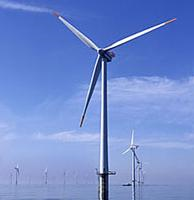
\includegraphics[scale=1]{figures/windmill.png}
	\caption{Write a self-explaining caption. Captions are important for the reports readability}
	%\label{my-label}
\end{figure}

\begin{minipage}{0.5\textwidth}

\begin{figure}[H]
	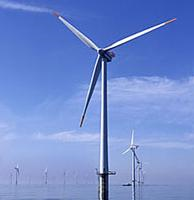
\includegraphics[scale=1]{figures/windmill.png}
	\caption{Example of two figure alligned side by side. Use a table as shown }
	%\label{my-label}
\end{figure}
\end{minipage} \hfill
\begin{minipage}{0.47\textwidth}
\begin{figure}[H]
	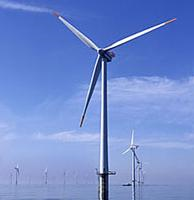
\includegraphics[scale=1]{figures/windmill.png}
	\caption{Example of two figures alligned side by side}
	%\label{my-label}
\end{figure}

\end{minipage}

Below with a vertical setup writing the Title above and the text describing the figure below.